\chapter{Analisi dei dati}

\section{Modifiche del pacchetto connectx}
Per confrontare le performance delle diverse AI, oltre al semplice torneo tra le varie versioni, si è ritenuto necessario apportare delle modifiche al pacchetto \verb!connectx!.
Più precisamente, all'interno dell'interfaccia \verb!connectx.CXPlayer! è stata introdotta una funzione \verb!Exit! che viene chiamata al termine di una partita fatta partire da \verb!connectx.CXPlayerTester!.
In questo modo, è risultato più semplice e veloce raccogliere i dati delle partite giocate.

Ogni versione della nostra AI infatti salva in un file \verb!.csv! vari dati relativi ad una partita giocata, tra cui:
\begin{itemize}
    \item il numero di nodi visitati;
    \item il numero di nodi valutati (foglie raggiunte);
    \item il numero di nodi tagliati (dall'alpha-beta pruning);
    \item il numero di nodi riutilizzati (transposition table hit);
\end{itemize}

Uno script in Python si occupa poi di leggere i file \verb!.csv! e di generare i grafici relativi ai dati raccolti, sia delle singole AI che di tutte le versioni confrontate tra loro, per ogni tipo di dato.

\section{Grafici}

Di seguito sono riportati i grafici delle singole AI e i confronti tra queste. Sono state omesse le ultime quattro configurazioni in quanto i dati da salvare facevano overflow sul dato \verb!long!.

\begin{center}
    \begin{figure}[!htb]
        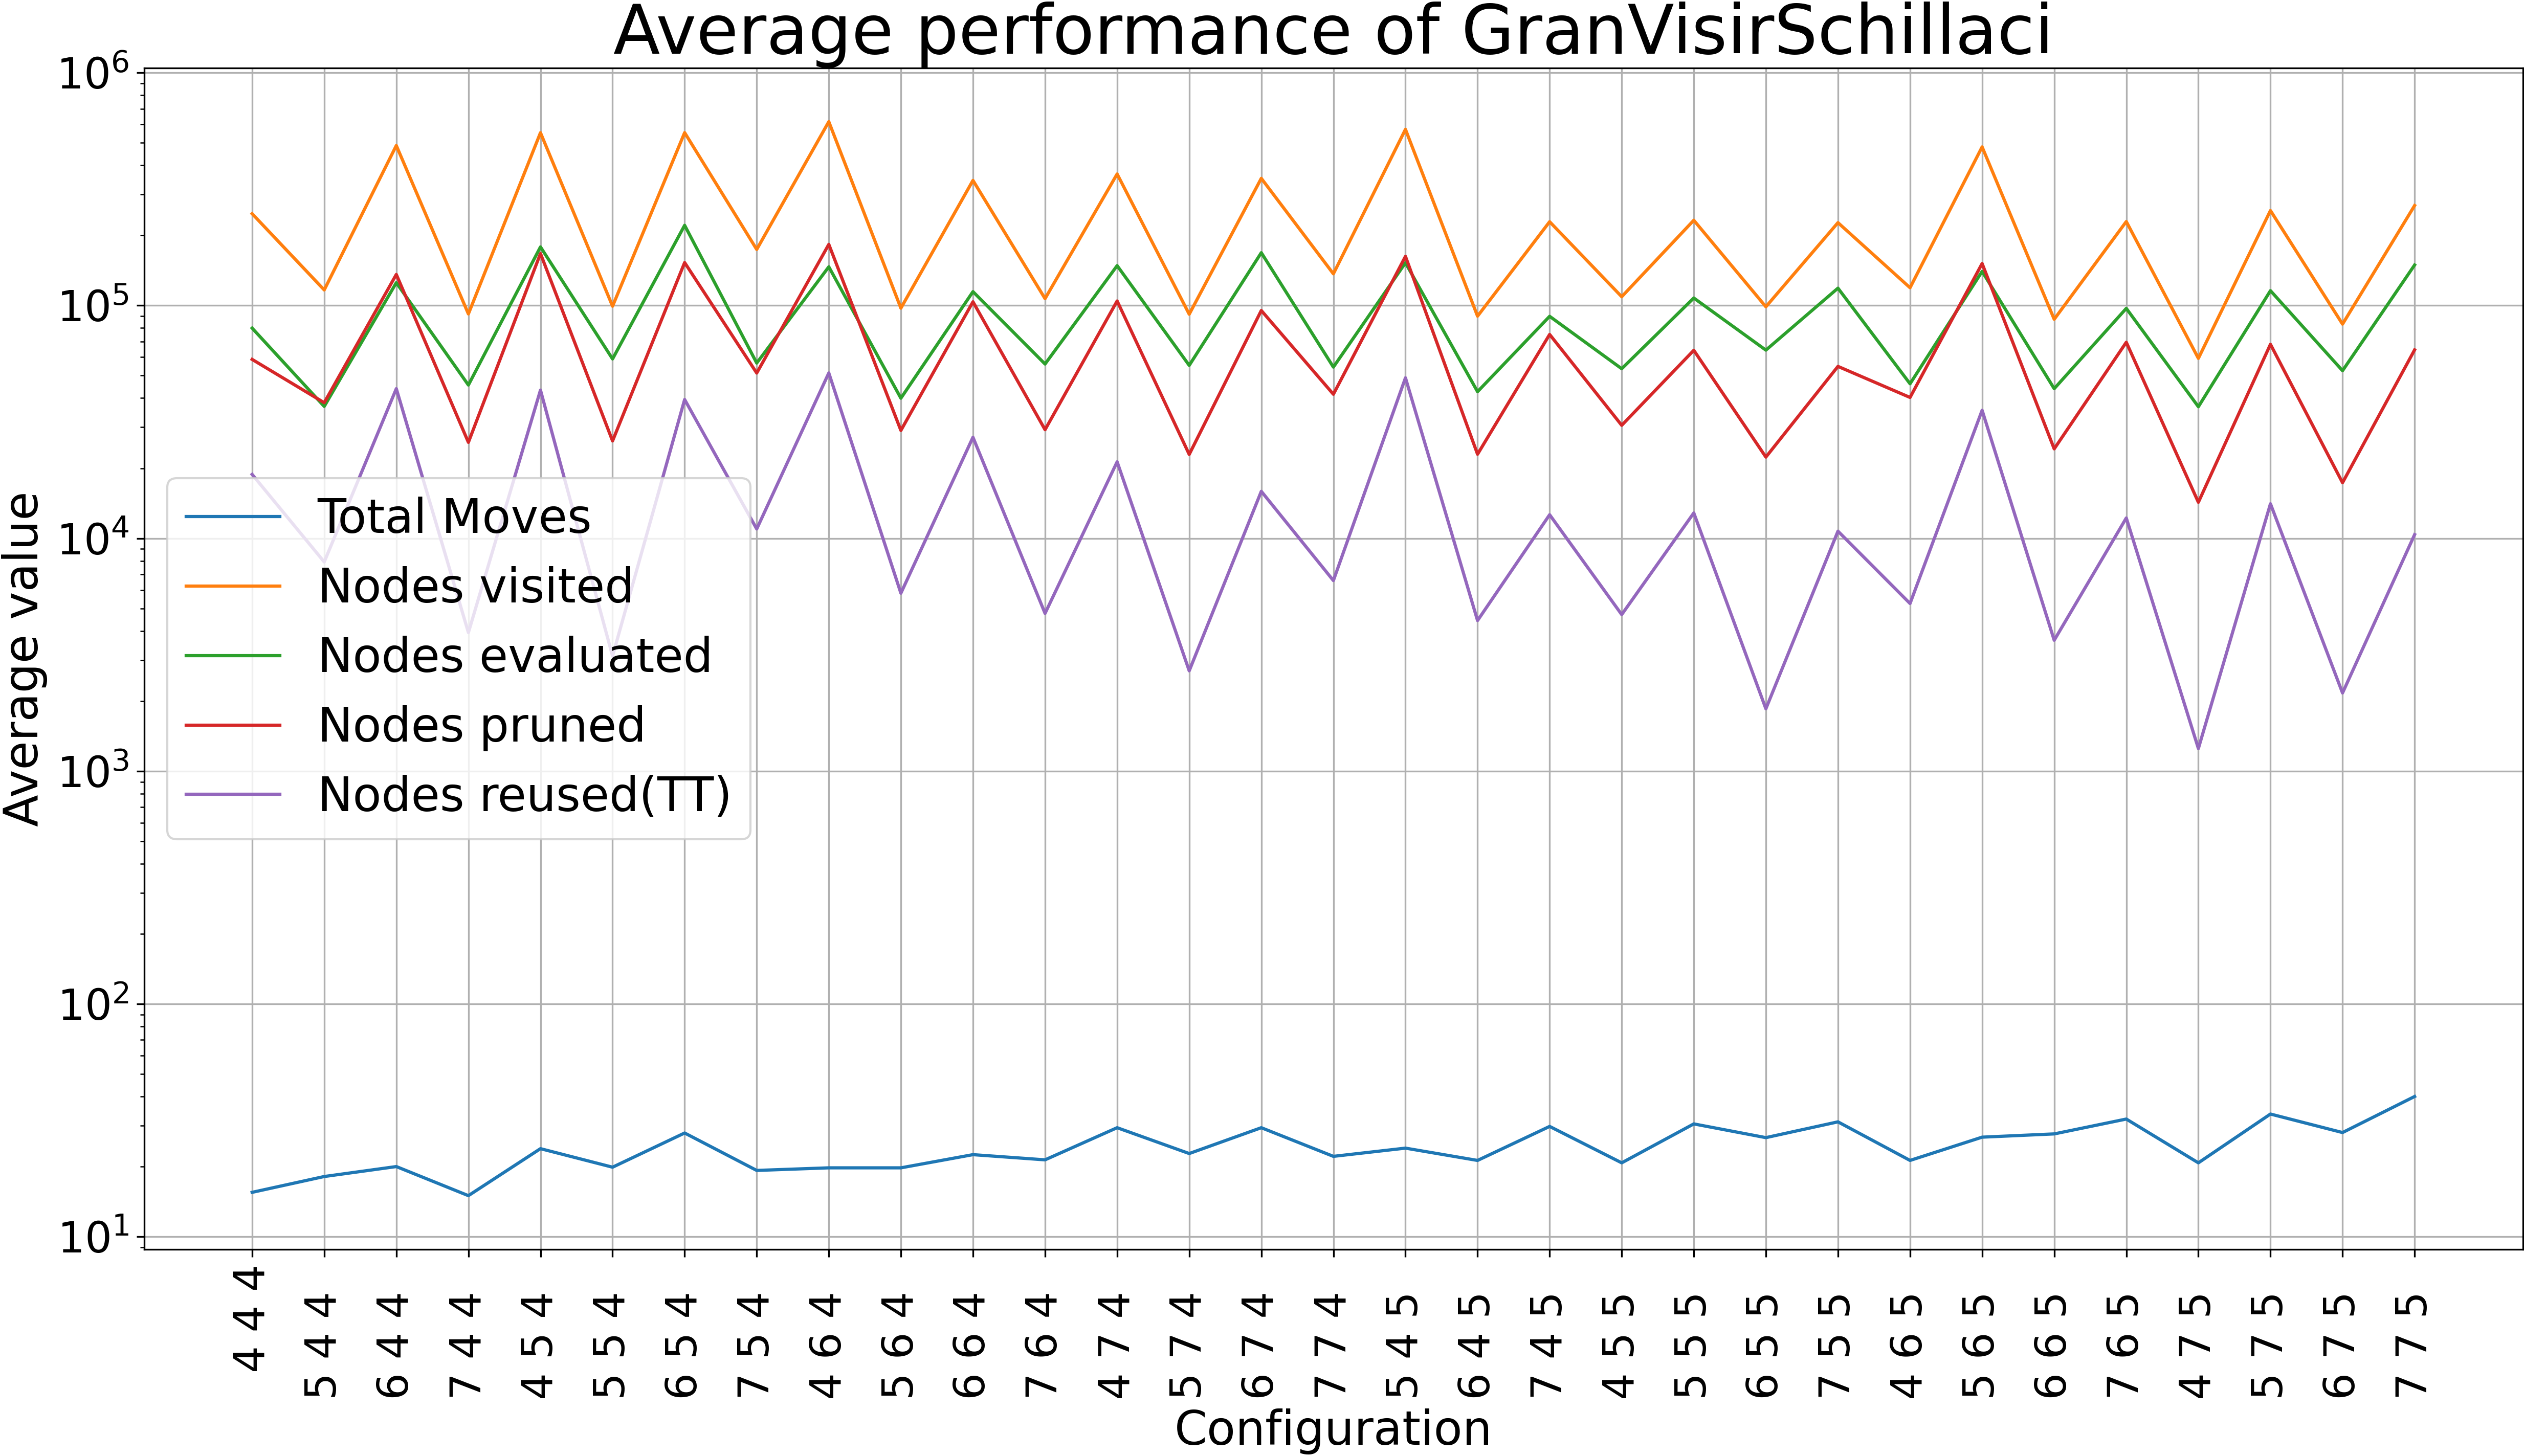
\includegraphics[width=0.9\textwidth]{images/plot_GranVisirSchillaci}


        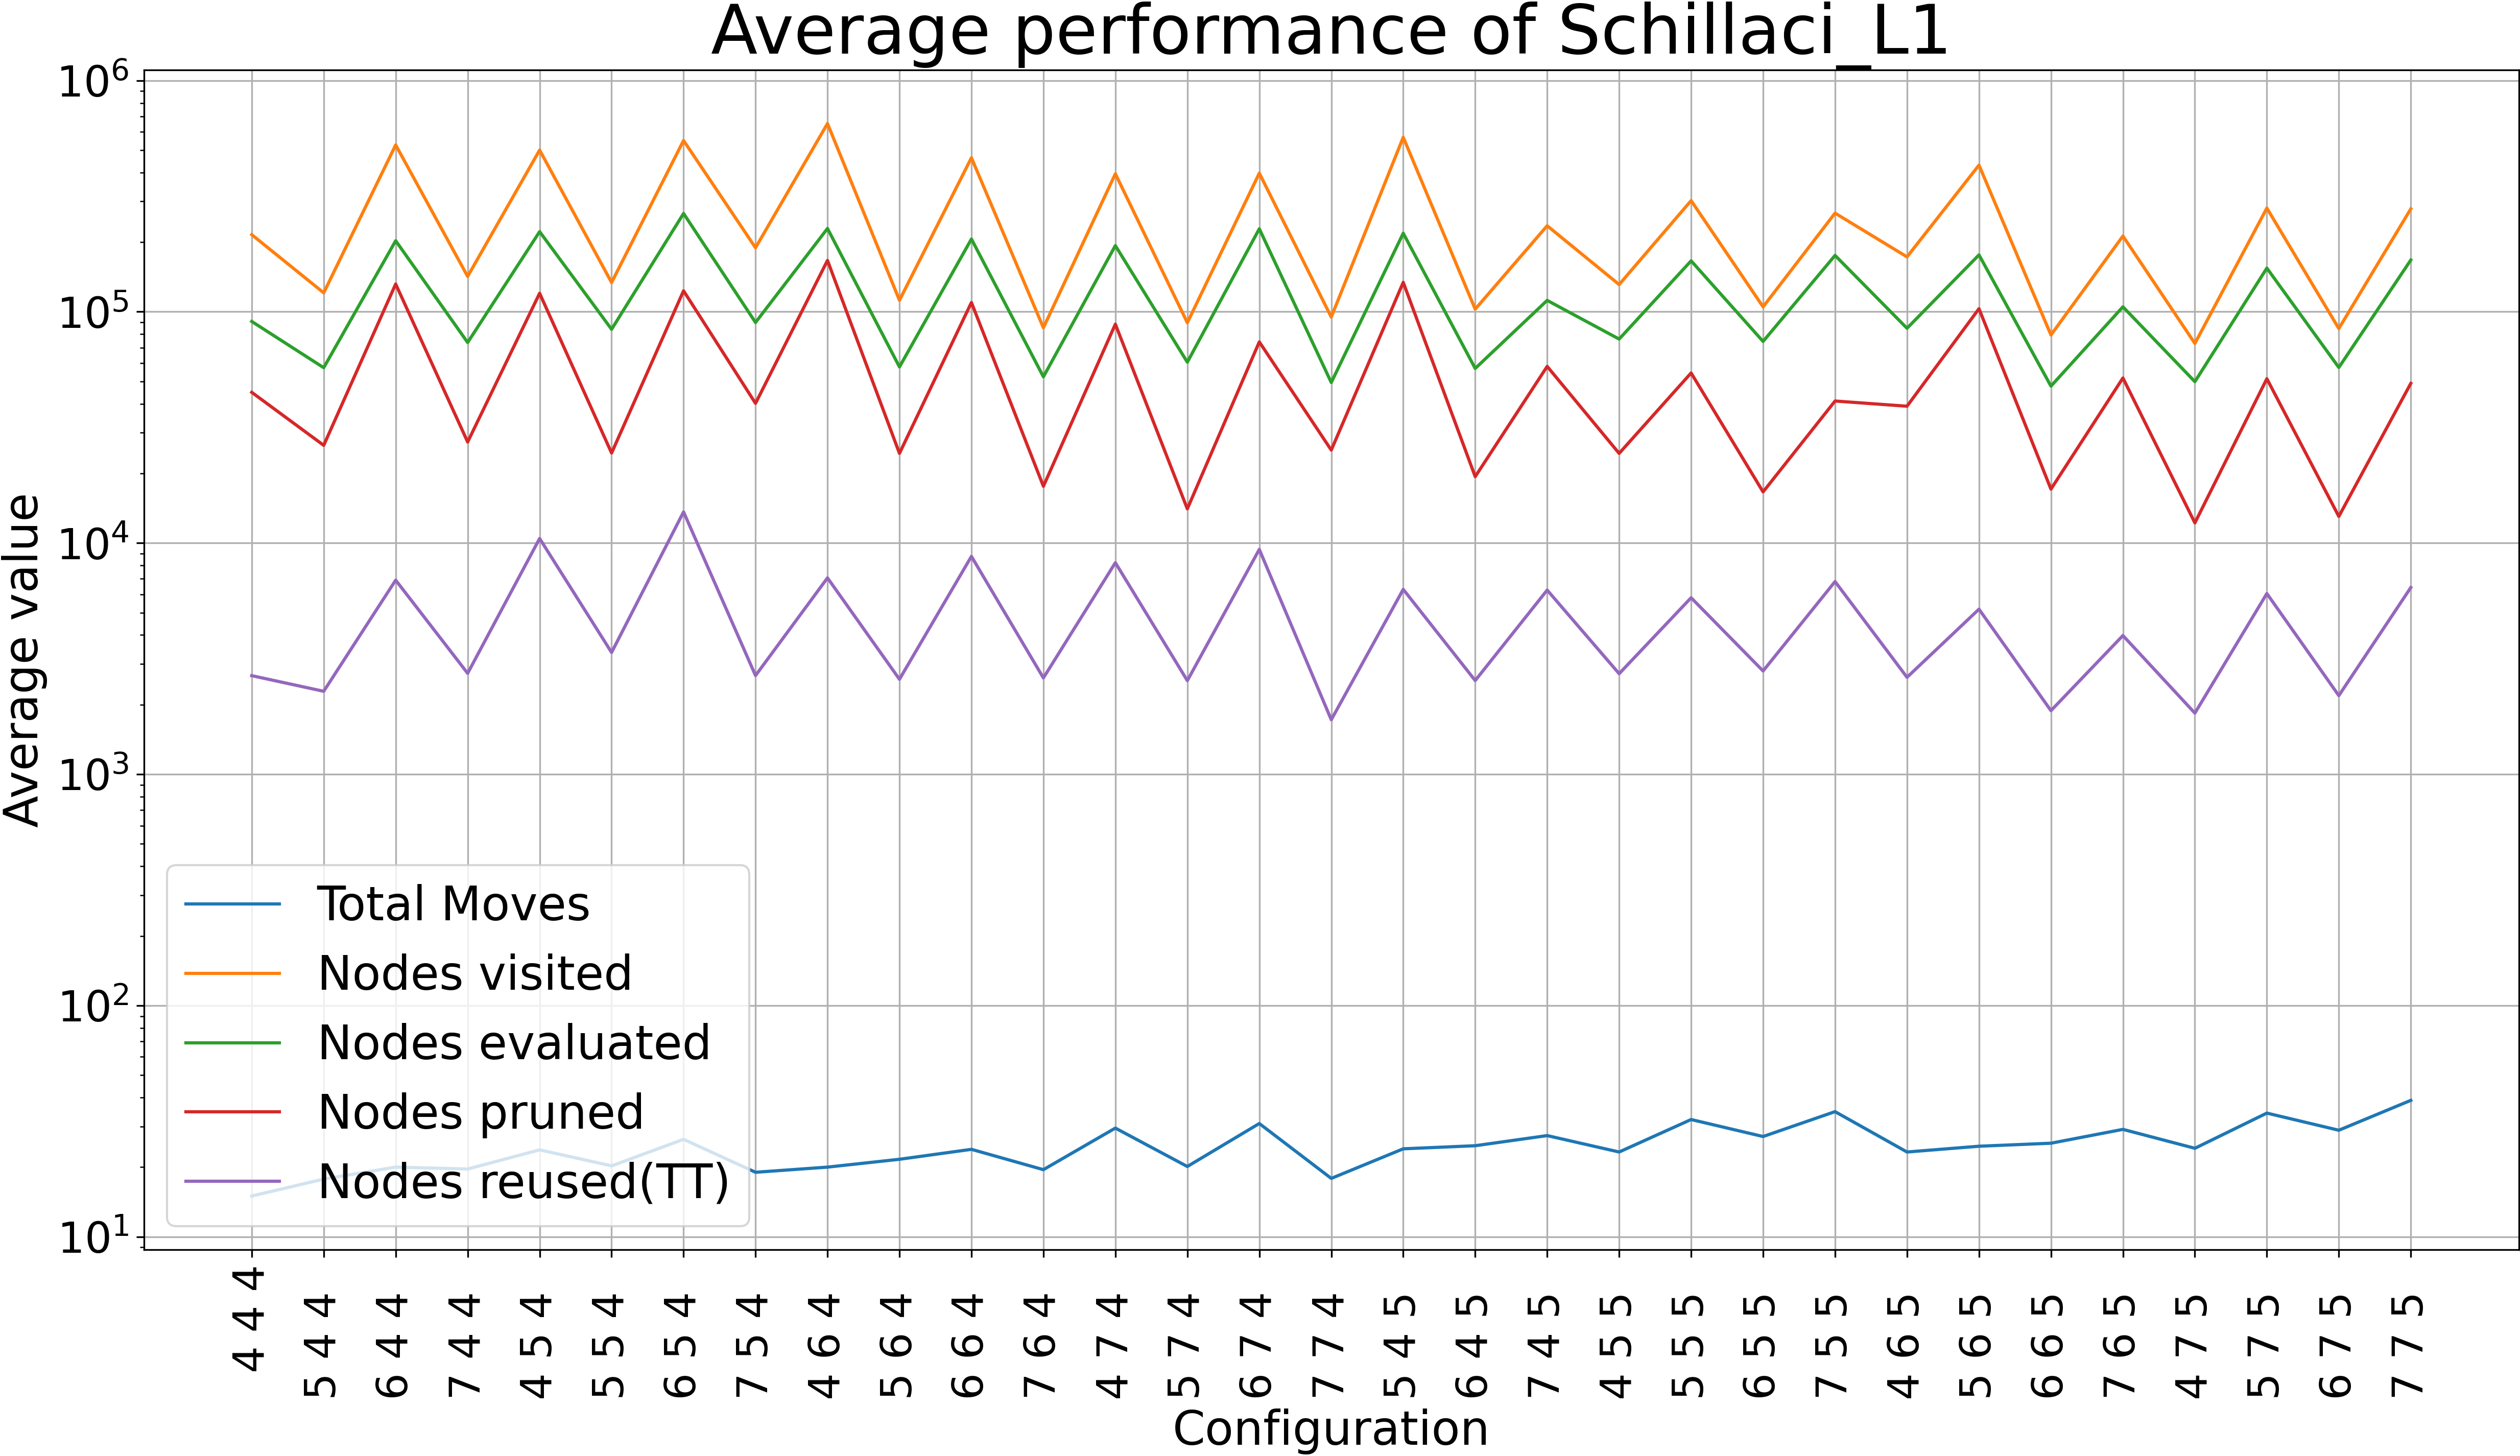
\includegraphics[width=0.9\textwidth]{images/plot_Schillaci_L1}


        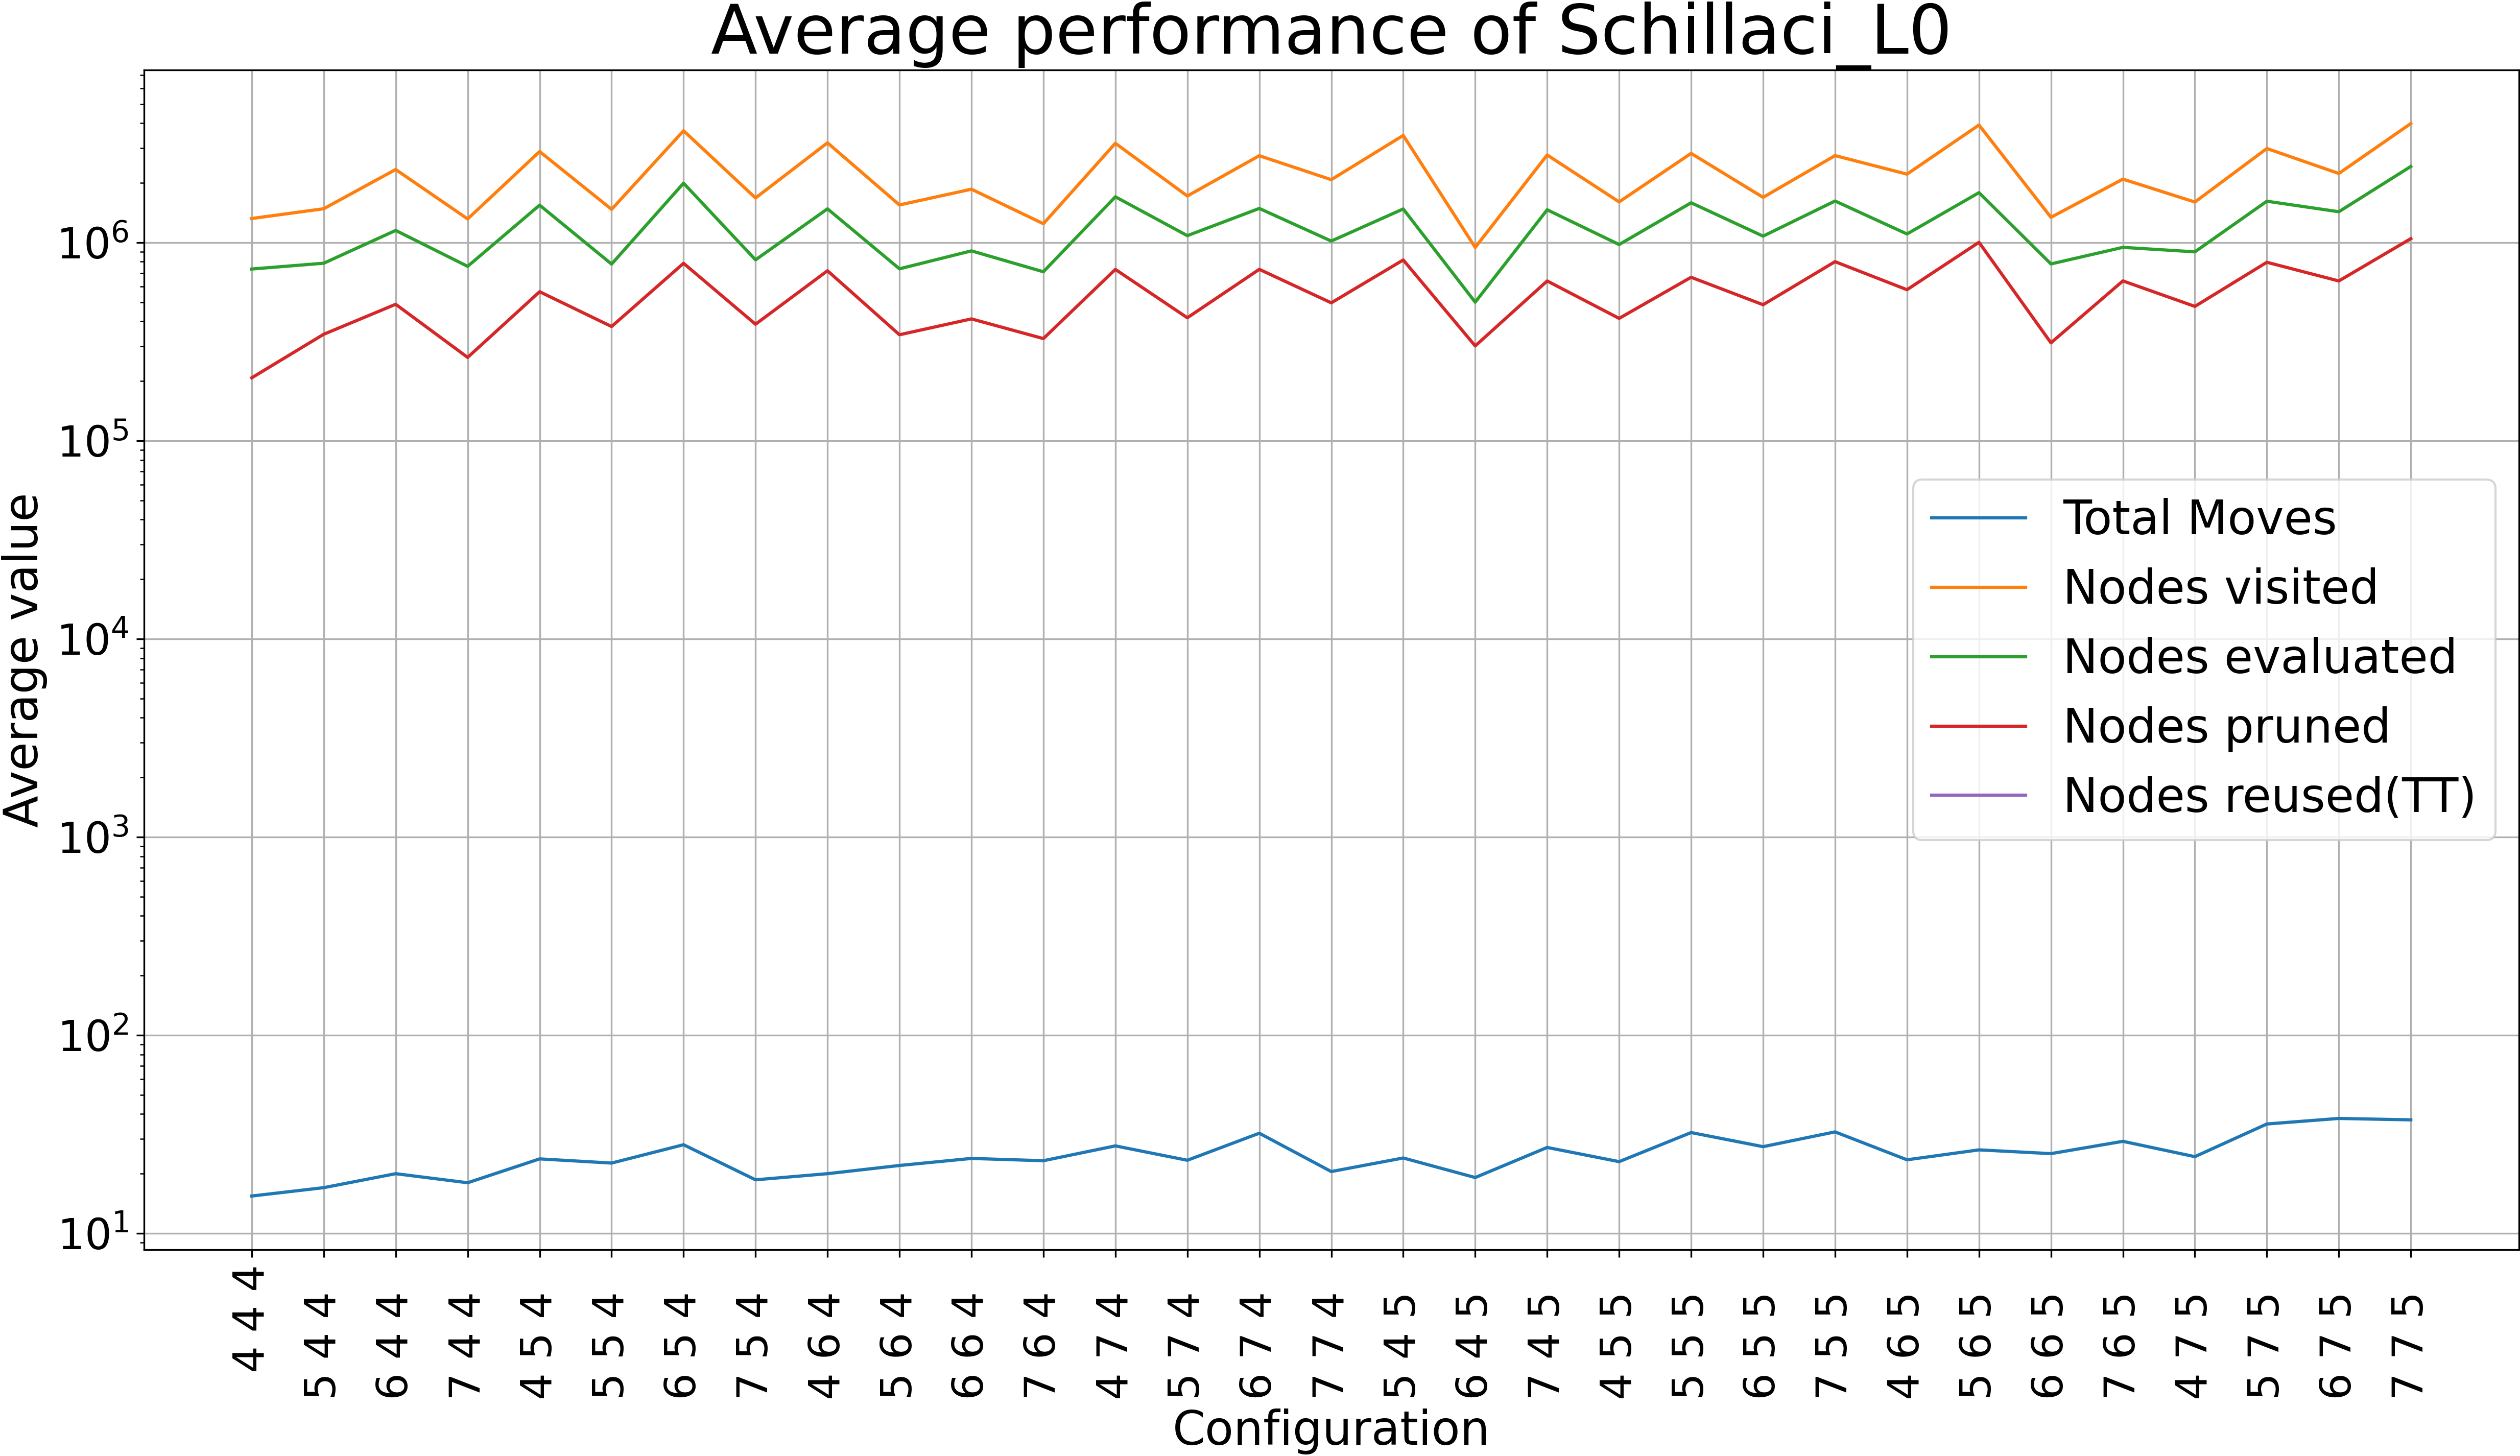
\includegraphics[width=0.9\textwidth]{images/plot_Schillaci_L0}
    \end{figure}
\end{center}

\begin{figure}[!htb]
    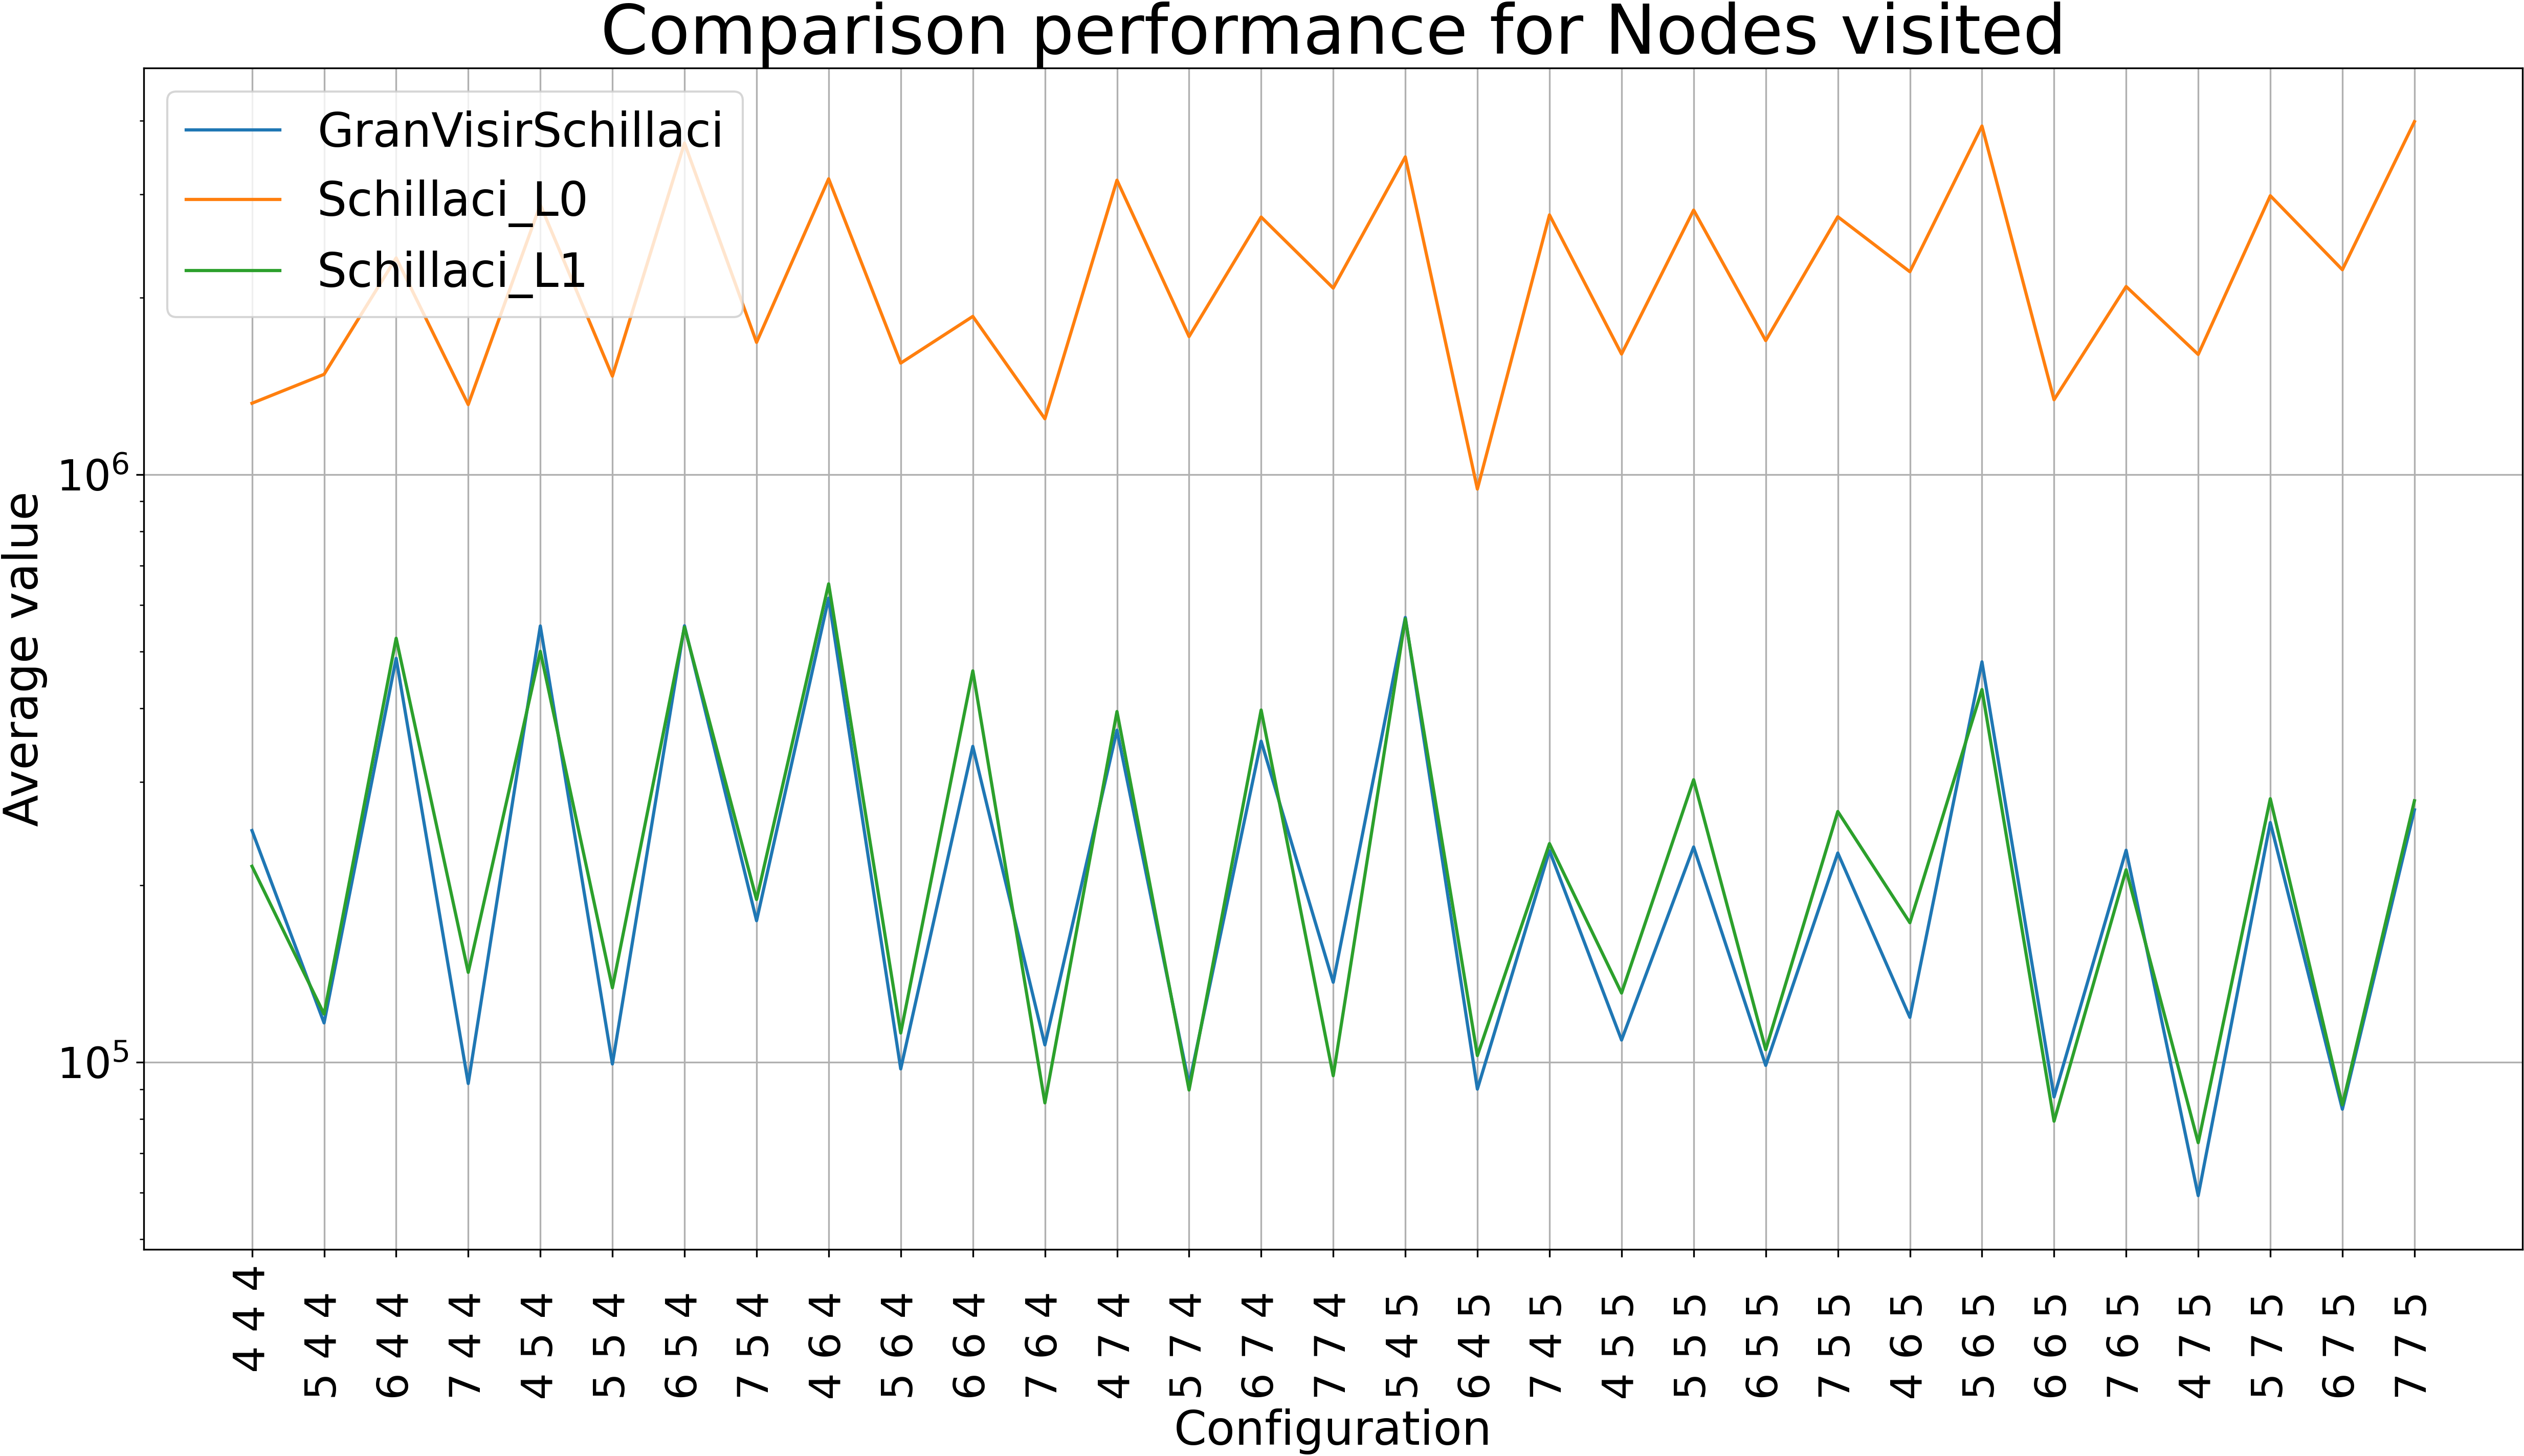
\includegraphics[width=0.9\textwidth]{../plots/plot_comparison_Nodes visited}


    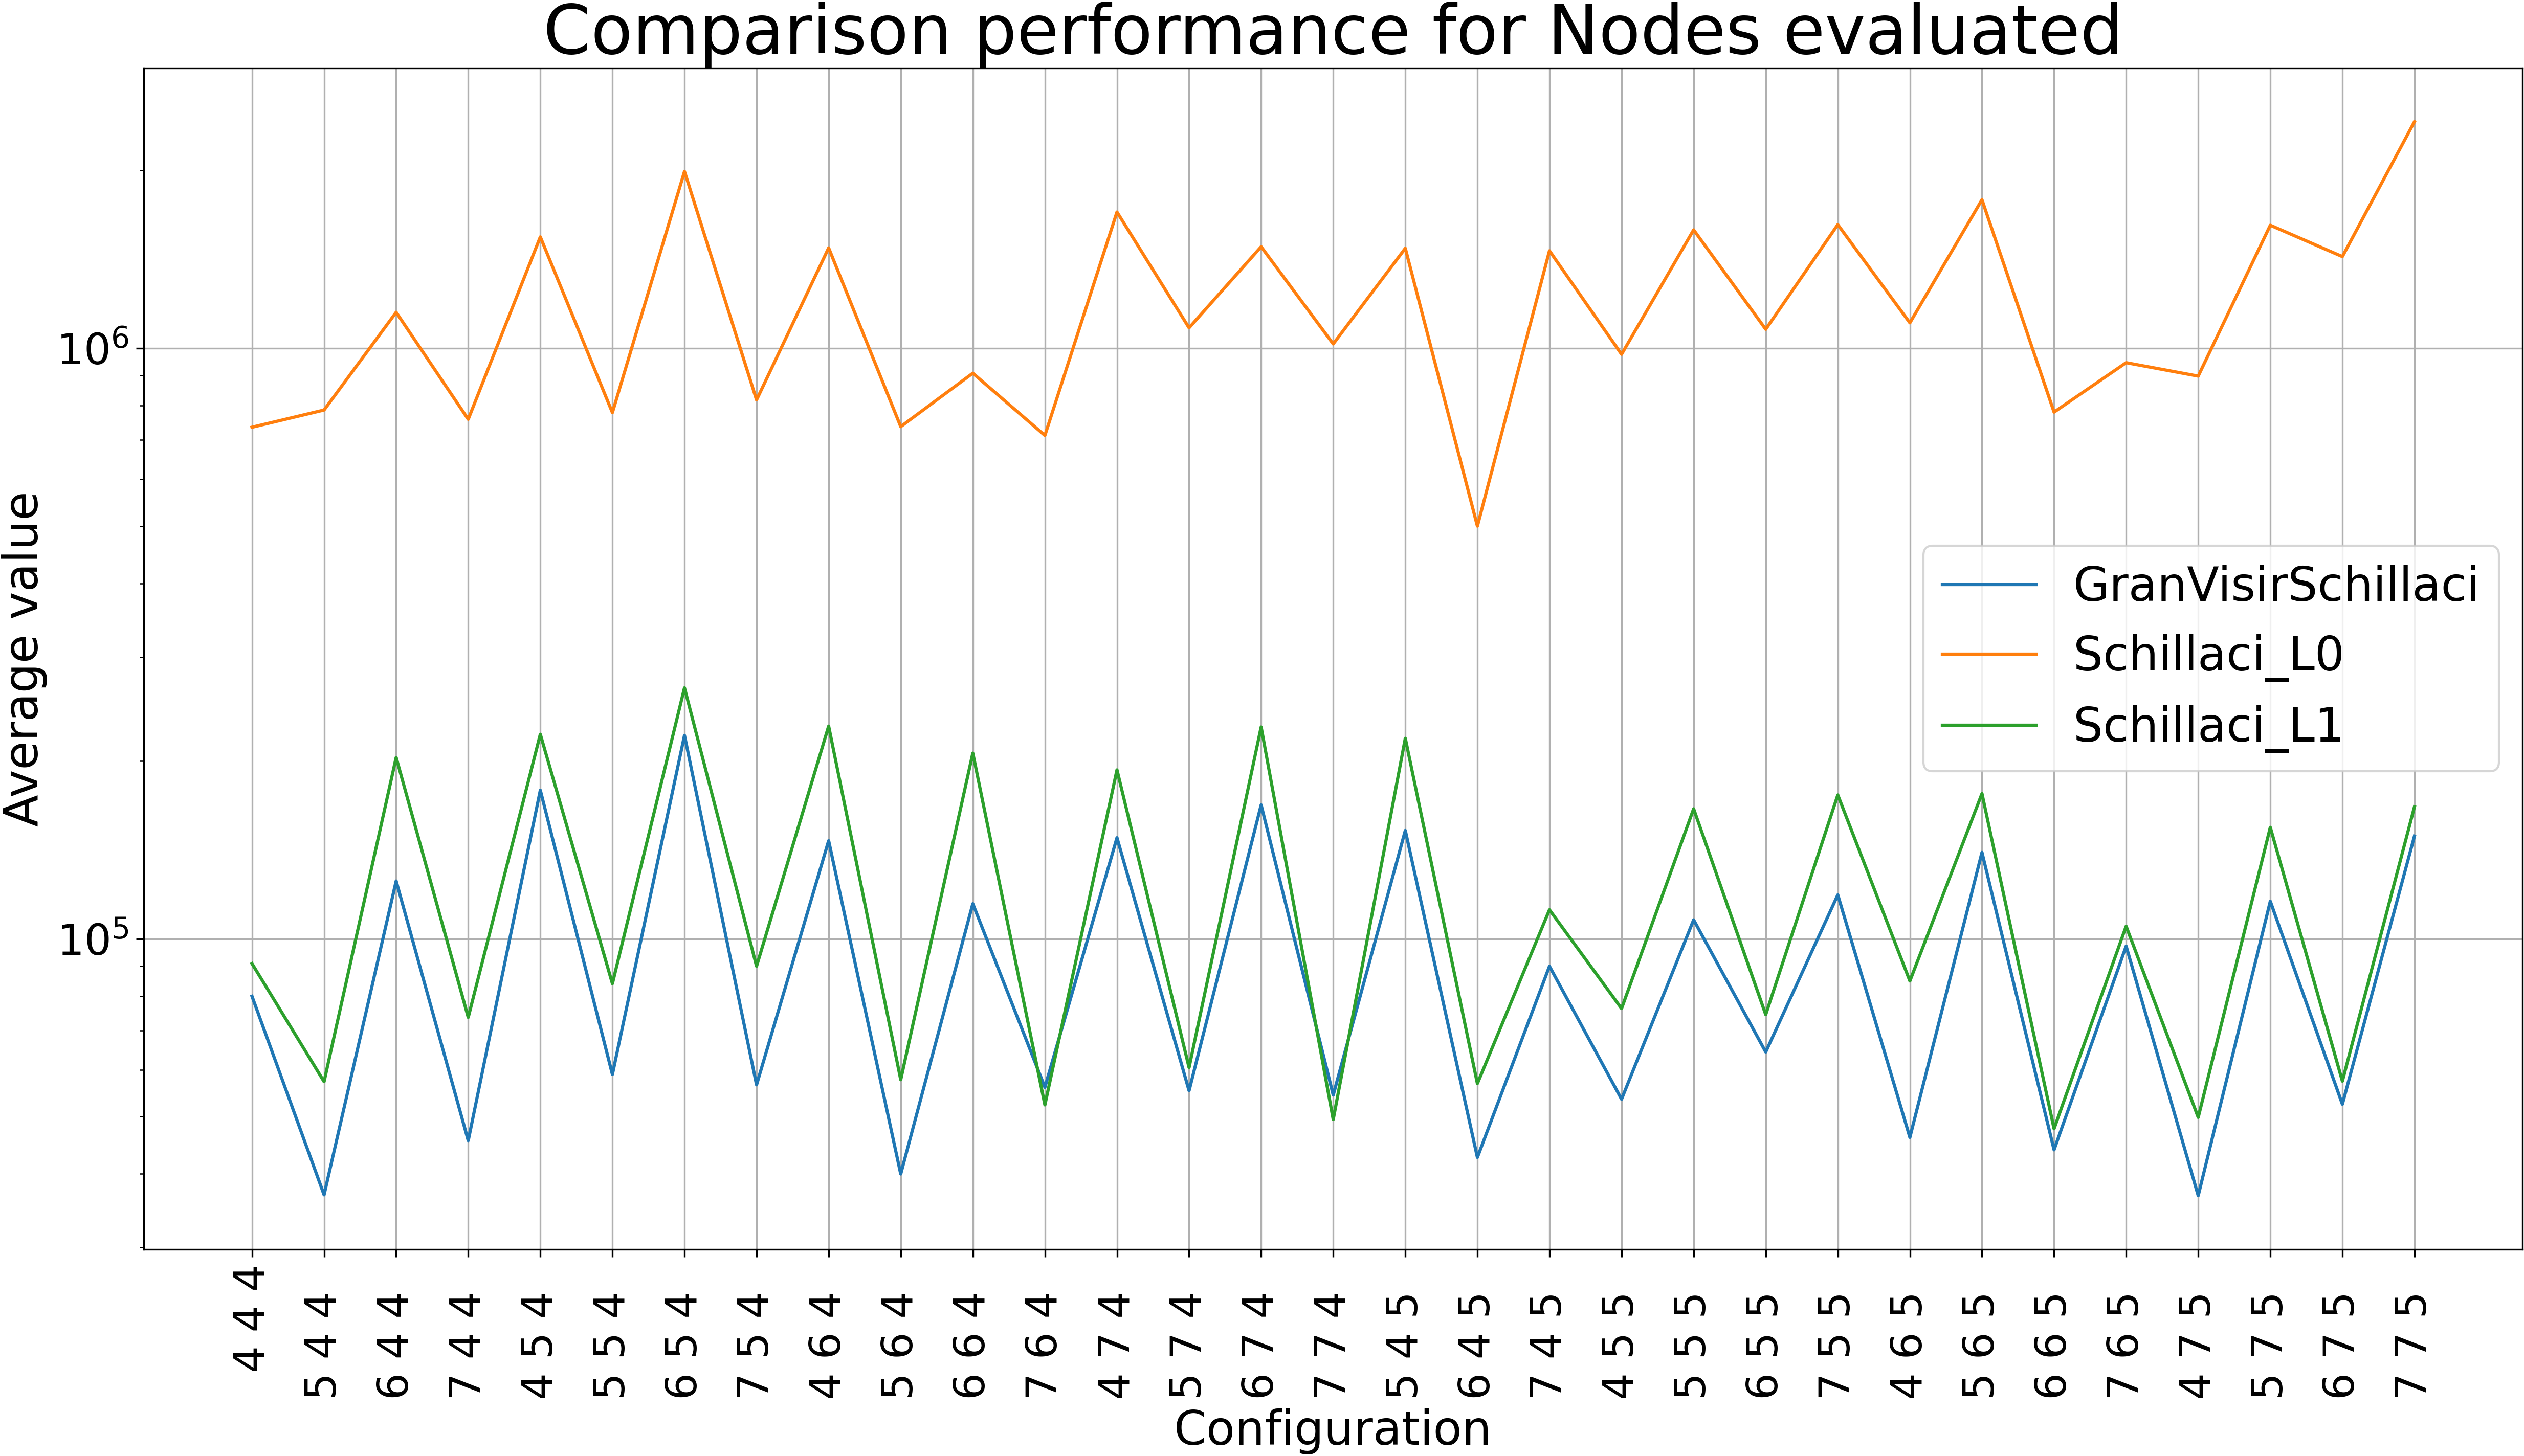
\includegraphics[width=0.9\textwidth]{../plots/plot_comparison_Nodes evaluated}
\end{figure}

\begin{figure}[!htb]
    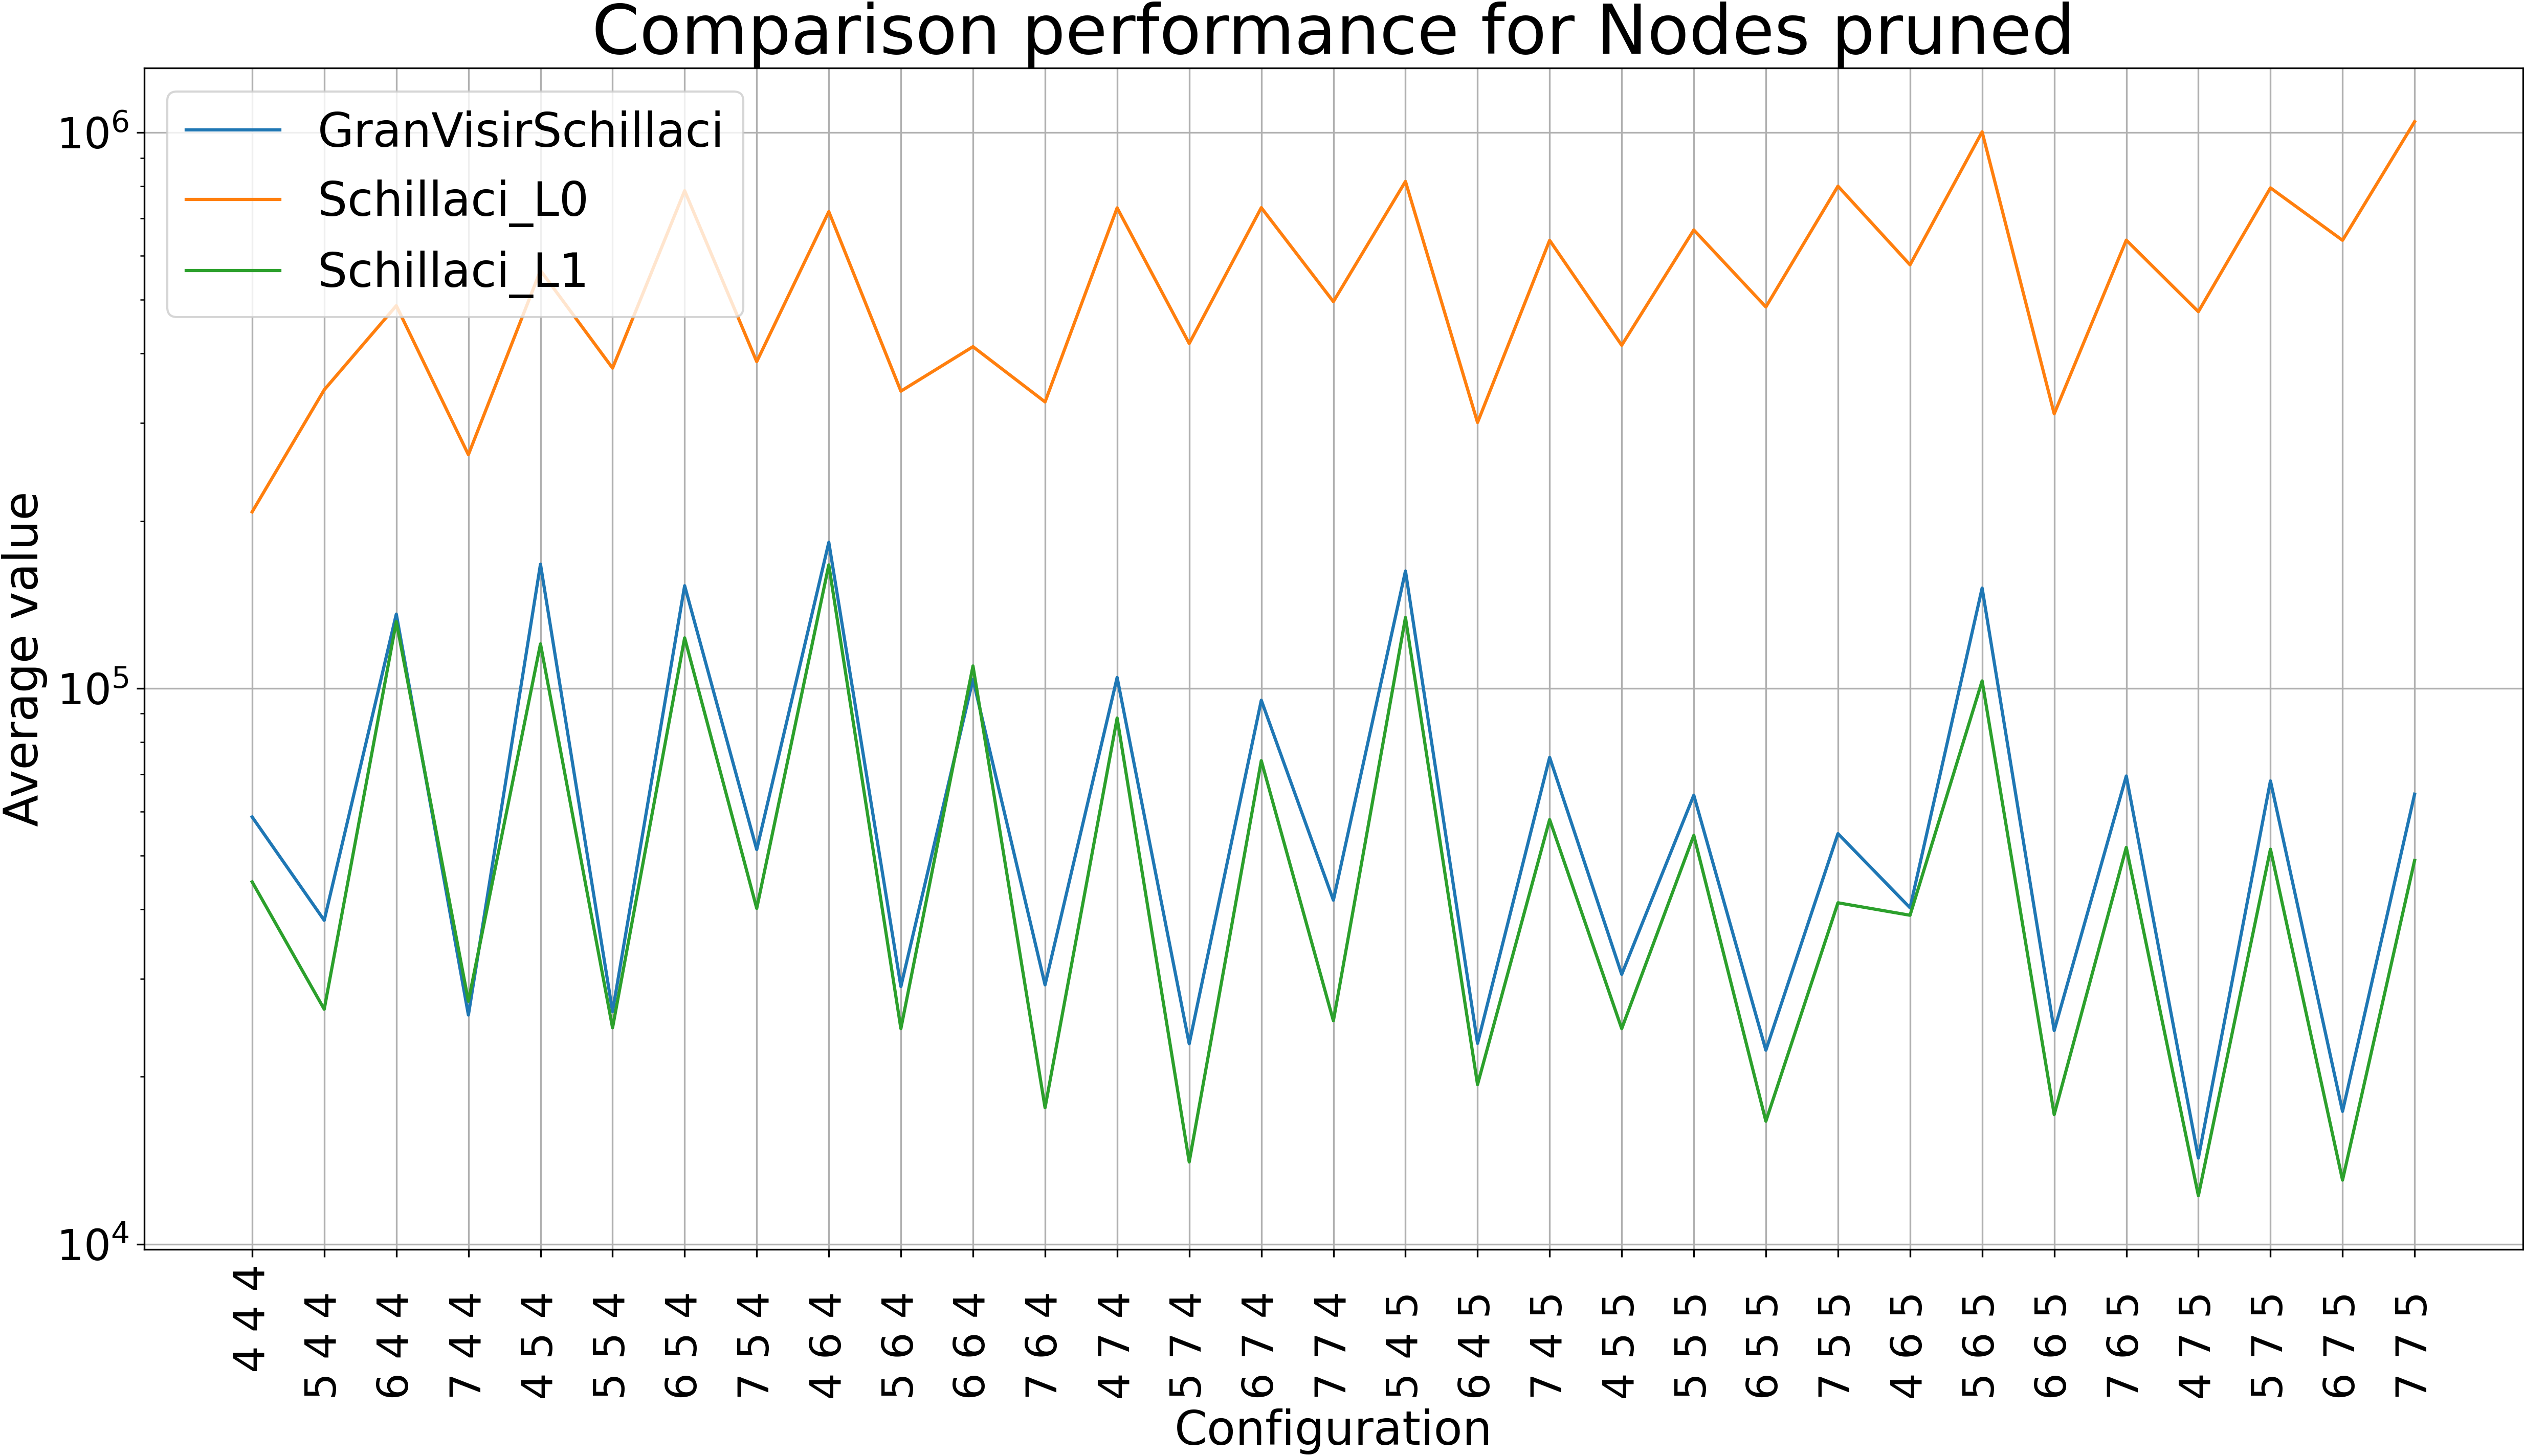
\includegraphics[width=0.9\textwidth]{../plots/plot_comparison_Nodes pruned}


    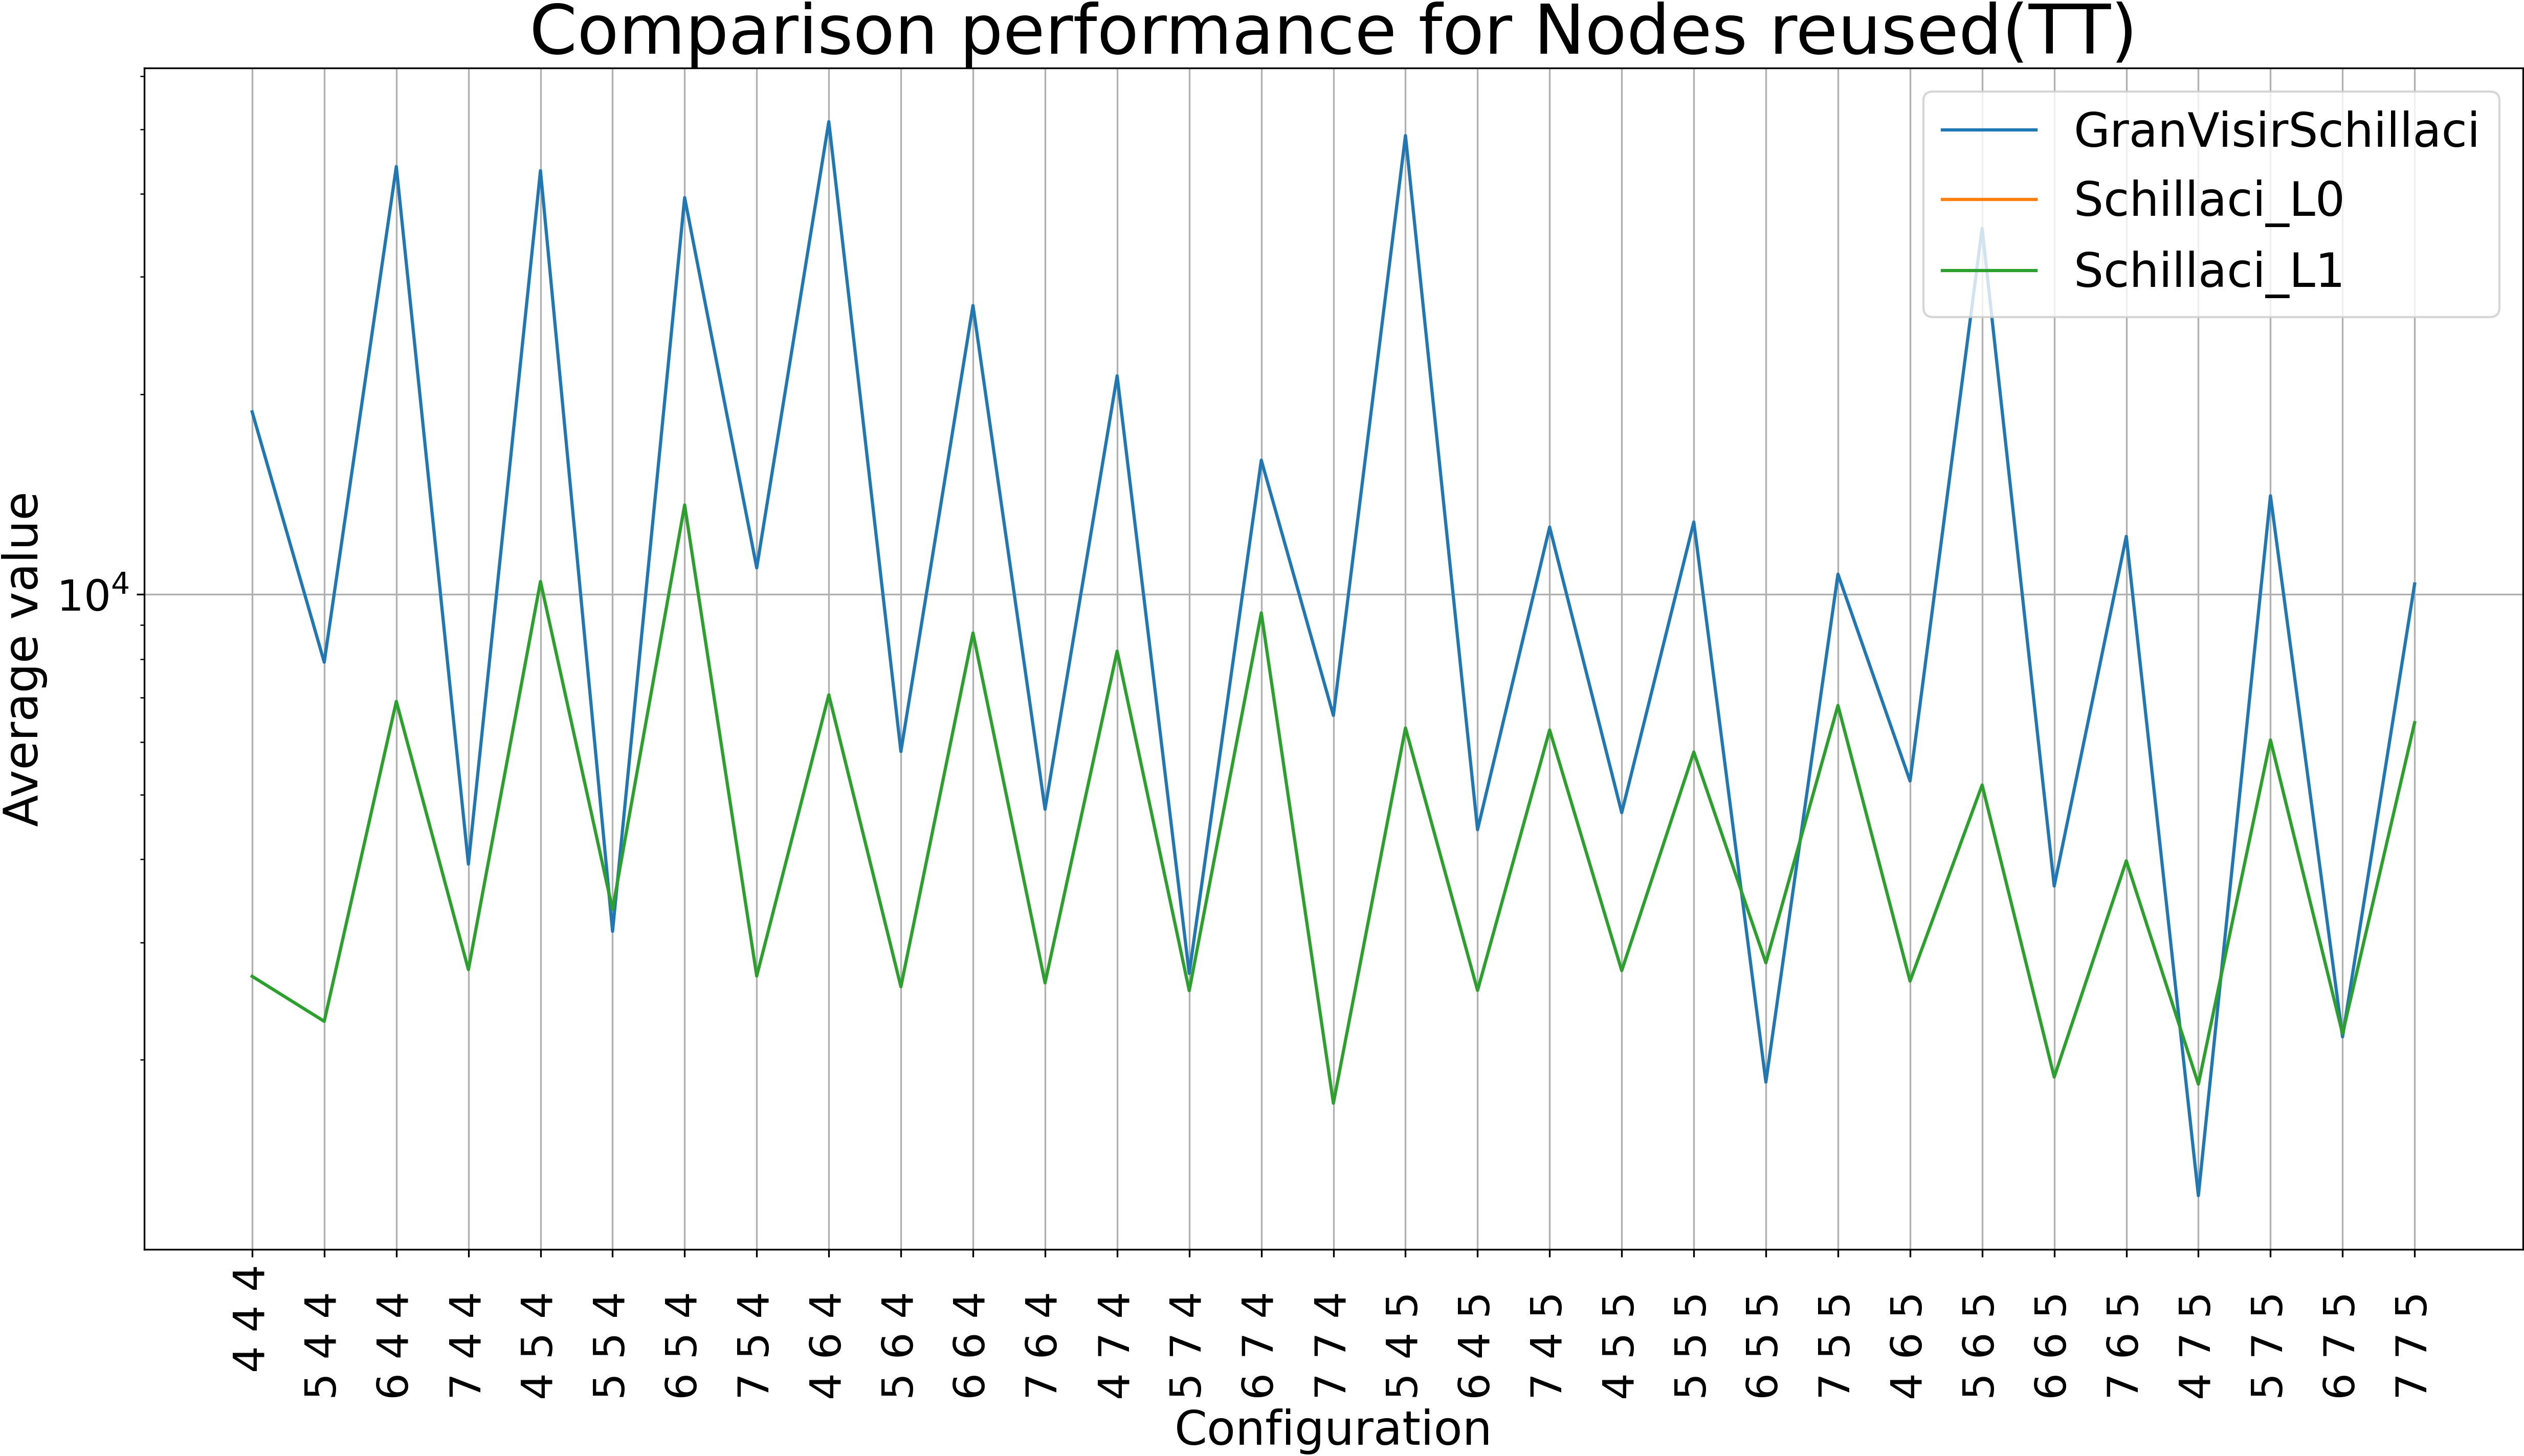
\includegraphics[width=0.9\textwidth]{../plots/plot_comparison_Nodes reused(TT)}
\end{figure}
